% Options for packages loaded elsewhere
\PassOptionsToPackage{unicode}{hyperref}
\PassOptionsToPackage{hyphens}{url}
\PassOptionsToPackage{space}{xeCJK}
%
\documentclass[
  10pt,
  ignorenonframetext,
  aspectratio=169,
  t]{beamer}
\usepackage{pgfpages}
\setbeamertemplate{caption}[numbered]
\setbeamertemplate{caption label separator}{: }
\setbeamercolor{caption name}{fg=normal text.fg}
\beamertemplatenavigationsymbolsempty
% Prevent slide breaks in the middle of a paragraph
\widowpenalties 1 10000
\raggedbottom
\setbeamertemplate{part page}{
  \centering
  \begin{beamercolorbox}[sep=16pt,center]{part title}
    \usebeamerfont{part title}\insertpart\par
  \end{beamercolorbox}
}
\setbeamertemplate{section page}{
  \centering
  \begin{beamercolorbox}[sep=12pt,center]{part title}
    \usebeamerfont{section title}\insertsection\par
  \end{beamercolorbox}
}
\setbeamertemplate{subsection page}{
  \centering
  \begin{beamercolorbox}[sep=8pt,center]{part title}
    \usebeamerfont{subsection title}\insertsubsection\par
  \end{beamercolorbox}
}
\AtBeginPart{
  \frame{\partpage}
}
\AtBeginSection{
  \ifbibliography
  \else
    \frame{\sectionpage}
  \fi
}
\AtBeginSubsection{
  \frame{\subsectionpage}
}
\usepackage{amsmath,amssymb}
\usepackage{iftex}
\ifPDFTeX
  \usepackage[T1]{fontenc}
  \usepackage[utf8]{inputenc}
  \usepackage{textcomp} % provide euro and other symbols
\else % if luatex or xetex
  \usepackage{unicode-math} % this also loads fontspec
  \defaultfontfeatures{Scale=MatchLowercase}
  \defaultfontfeatures[\rmfamily]{Ligatures=TeX,Scale=1}
\fi
\usepackage{lmodern}
\usetheme[]{Madrid}
\usefonttheme{serif} % use mainfont rather than sansfont for slide text
\ifPDFTeX\else
  % xetex/luatex font selection
  \setmainfont[]{DejaVu Sans}
  \setmonofont[]{DejaVu Sans Mono}
  \ifXeTeX
    \usepackage{xeCJK}
    \setCJKmainfont[]{Noto Serif CJK SC}
          \fi
  \ifLuaTeX
    \usepackage[]{luatexja-fontspec}
    \setmainjfont[]{Noto Serif CJK SC}
  \fi
\fi
% Use upquote if available, for straight quotes in verbatim environments
\IfFileExists{upquote.sty}{\usepackage{upquote}}{}
\IfFileExists{microtype.sty}{% use microtype if available
  \usepackage[]{microtype}
  \UseMicrotypeSet[protrusion]{basicmath} % disable protrusion for tt fonts
}{}
\makeatletter
\@ifundefined{KOMAClassName}{% if non-KOMA class
  \IfFileExists{parskip.sty}{%
    \usepackage{parskip}
  }{% else
    \setlength{\parindent}{0pt}
    \setlength{\parskip}{6pt plus 2pt minus 1pt}}
}{% if KOMA class
  \KOMAoptions{parskip=half}}
\makeatother
\usepackage{xcolor}
\newif\ifbibliography
\usepackage{longtable,booktabs,array}
\usepackage{calc} % for calculating minipage widths
\usepackage{caption}
% Make caption package work with longtable
\makeatletter
\def\fnum@table{\tablename~\thetable}
\makeatother
\usepackage{graphicx}
\makeatletter
\def\maxwidth{\ifdim\Gin@nat@width>\linewidth\linewidth\else\Gin@nat@width\fi}
\def\maxheight{\ifdim\Gin@nat@height>\textheight\textheight\else\Gin@nat@height\fi}
\makeatother
% Scale images if necessary, so that they will not overflow the page
% margins by default, and it is still possible to overwrite the defaults
% using explicit options in \includegraphics[width, height, ...]{}
\setkeys{Gin}{width=\maxwidth,height=\maxheight,keepaspectratio}
% Set default figure placement to htbp
\makeatletter
\def\fps@figure{htbp}
\makeatother
\setlength{\emergencystretch}{3em} % prevent overfull lines
\providecommand{\tightlist}{%
  \setlength{\itemsep}{0pt}\setlength{\parskip}{0pt}}
\setcounter{secnumdepth}{-\maxdimen} % remove section numbering
% Tighten vertical rhythm so dense slides fit on a single frame.
\usepackage{etoolbox}
\setlength{\parskip}{3pt plus 1pt minus 1pt}
\setbeamertemplate{itemize/enumerate body begin}{\small}
\setbeamertemplate{itemize/enumerate subbody begin}{\footnotesize}
\AtBeginEnvironment{itemize}{\setlength{\itemsep}{2pt}\setlength{\topsep}{2pt}}
\AtBeginEnvironment{enumerate}{\setlength{\itemsep}{2pt}\setlength{\topsep}{2pt}}
% Shrink code listings and tables so long lines do not force a page break.
\AtBeginEnvironment{Highlighting}{\footnotesize}
\AtBeginEnvironment{verbatim}{\footnotesize}
\AtBeginEnvironment{longtable}{\scriptsize}
\ifLuaTeX
  \usepackage{selnolig}  % disable illegal ligatures
\fi
\IfFileExists{bookmark.sty}{\usepackage{bookmark}}{\usepackage{hyperref}}
\IfFileExists{xurl.sty}{\usepackage{xurl}}{} % add URL line breaks if available
\urlstyle{same}
\hypersetup{
  pdftitle={Scaling lanes on AgentCore: harness, inference and sandbox scaled together},
  pdfauthor={Kaige Yang --- Senior Applied Scientist, AWS},
  hidelinks,
  pdfcreator={LaTeX via pandoc}}

\title[Scaling lanes on AgentCore]{Scaling lanes on AgentCore: harness, inference and sandbox scaled
together}
\author[Kaige Yang, AWS]{Kaige Yang --- Senior Applied Scientist, AWS}
\date{September 24, 2026}

\setbeamertemplate{frametitle continuation}[from second]
\begin{document}
\frame{\titlepage}

\begin{frame}[fragile]{Summary}
\protect\hypertarget{summary}{}
\begin{longtable}[]{@{}
  >{\raggedright\arraybackslash}p{(\columnwidth - 2\tabcolsep) * \real{0.1522}}
  >{\raggedright\arraybackslash}p{(\columnwidth - 2\tabcolsep) * \real{0.8478}}@{}}
\caption{The deck in one table}\tabularnewline
\toprule\noalign{}
\endfirsthead
\endhead
\textbf{Goal} & Scale an agentic-RL rollout (slime GRPO, Qwen3-4B) by
scaling \textbf{all three tiers} together: harness, inference,
sandbox \\
\textbf{Challenge} & Throughput = \textbf{min(inference, sandbox,
harness)}. A single harness is a hidden ceiling, the router scatters an
episode's turns, and a fresh session per episode puts an open on every
episode \\
\textbf{Solution} & \textbf{Lanes, 1 : 1 : 1:} W warm harness workers,
each pinned to its own SGLang engine and its own \textbf{persistent
AgentCore microVM}, with a fresh workdir per episode \\
\textbf{Result} & Smoke run on AWS (4 × 4 × 4): 400 episodes, lanes
verified 1:1:1, \textbf{4 session opens instead of 400}, sandbox p95
\textbf{431 → 120 ms}. Rollout time unchanged: this task is
\textbf{inference-bound} \\
\bottomrule\noalign{}
\end{longtable}

Source: \texttt{code/demos/demo\_cpu\_scale\_lanes/},
\texttt{docs/harness-scaling.md}.
\end{frame}

\hypertarget{agentcore-seen-from-agentic-rl}{%
\section{1 · AgentCore, seen from agentic
RL}\label{agentcore-seen-from-agentic-rl}}

\begin{frame}[fragile]{Where AgentCore sits in the RL loop}
\protect\hypertarget{where-agentcore-sits-in-the-rl-loop}{}
An agentic-RL rollout is produced by \textbf{three replicated tiers}.
AgentCore is the \textbf{sandbox} tier.

\begin{longtable}[]{@{}
  >{\raggedright\arraybackslash}p{(\columnwidth - 4\tabcolsep) * \real{0.1682}}
  >{\raggedright\arraybackslash}p{(\columnwidth - 4\tabcolsep) * \real{0.4486}}
  >{\raggedright\arraybackslash}p{(\columnwidth - 4\tabcolsep) * \real{0.3832}}@{}}
\caption{The three tiers}\tabularnewline
\toprule\noalign{}
\begin{minipage}[b]{\linewidth}\raggedright
RL tier
\end{minipage} & \begin{minipage}[b]{\linewidth}\raggedright
Role in the episode
\end{minipage} & \begin{minipage}[b]{\linewidth}\raggedright
In this demo
\end{minipage} \\
\midrule\noalign{}
\endfirsthead
\toprule\noalign{}
\begin{minipage}[b]{\linewidth}\raggedright
RL tier
\end{minipage} & \begin{minipage}[b]{\linewidth}\raggedright
Role in the episode
\end{minipage} & \begin{minipage}[b]{\linewidth}\raggedright
In this demo
\end{minipage} \\
\midrule\noalign{}
\endhead
\textbf{Harness} & Runs the agent loop: prompt → model → tool call →
observation → \ldots{} → reward & \texttt{MiniClaudeHarness}, in the
slime rollout process \\
\textbf{Inference} & The \textbf{policy under training}; every model
call is a sample we train on & SGLang engines, weights synced from slime
each step \\
\textbf{Sandbox} & The \textbf{environment}: executes the agent's tool
calls, holds its files, runs the checker & \textbf{AgentCore Runtime
microVMs} \\
\bottomrule\noalign{}
\end{longtable}

\begin{itemize}
\tightlist
\item
  slime only sees \texttt{generate()} → a scored trajectory. Tiers are
  wired in through its \textbf{custom generate hook}, no slime fork.
\item
  \textbf{Throughput = min(inference, sandbox, harness)}: scale one tier
  alone and the smallest one caps the rollout.
\end{itemize}
\end{frame}

\begin{frame}[fragile]{Three AgentCore concepts, and what each means for
RL}
\protect\hypertarget{three-agentcore-concepts-and-what-each-means-for-rl}{}
\begin{longtable}[]{@{}
  >{\raggedright\arraybackslash}p{(\columnwidth - 4\tabcolsep) * \real{0.1964}}
  >{\raggedright\arraybackslash}p{(\columnwidth - 4\tabcolsep) * \real{0.4286}}
  >{\raggedright\arraybackslash}p{(\columnwidth - 4\tabcolsep) * \real{0.3750}}@{}}
\caption{Runtime 1 : N sessions, session 1 : 1 microVM}\tabularnewline
\toprule\noalign{}
\begin{minipage}[b]{\linewidth}\raggedright
AgentCore
\end{minipage} & \begin{minipage}[b]{\linewidth}\raggedright
What it is
\end{minipage} & \begin{minipage}[b]{\linewidth}\raggedright
RL meaning
\end{minipage} \\
\midrule\noalign{}
\endfirsthead
\toprule\noalign{}
\begin{minipage}[b]{\linewidth}\raggedright
AgentCore
\end{minipage} & \begin{minipage}[b]{\linewidth}\raggedright
What it is
\end{minipage} & \begin{minipage}[b]{\linewidth}\raggedright
RL meaning
\end{minipage} \\
\midrule\noalign{}
\endhead
\textbf{Runtime} (ARN) & A template: one container image + entry point &
An \textbf{environment type} (tool set, OS, packages). One per image,
not per task \\
\textbf{Session} (\texttt{runtimeSessionId}) & The routing key; same id
→ same VM & An \textbf{episode's handle}: sticky for the episode's
life \\
\textbf{microVM} & Firecracker VM (2 vCPU, 8 GB), 1 : 1 with a session &
The \textbf{isolation boundary}: a new session is a clean reset \\
\bottomrule\noalign{}
\end{longtable}

\begin{itemize}
\tightlist
\item
  \textbf{No ``create session'' call:} the first invoke with a new id
  \textbf{is} the boot (cold ≈ seconds, warm hit ≈ 0.5 s).
\item
  \textbf{Reset = a new session.} \texttt{StopRuntimeSession} terminates
  and sanitises the VM.
\item
  One Runtime serves many concurrent sessions, so \textbf{GRPO siblings
  share a Runtime but never a VM}.
\end{itemize}
\end{frame}

\begin{frame}{The lifecycle, read as rollout costs}
\protect\hypertarget{the-lifecycle-read-as-rollout-costs}{}
\begin{longtable}[]{@{}
  >{\raggedright\arraybackslash}p{(\columnwidth - 2\tabcolsep) * \real{0.4356}}
  >{\raggedright\arraybackslash}p{(\columnwidth - 2\tabcolsep) * \real{0.5644}}@{}}
\caption{Lifecycle → cost}\tabularnewline
\toprule\noalign{}
\begin{minipage}[b]{\linewidth}\raggedright
AgentCore behaviour
\end{minipage} & \begin{minipage}[b]{\linewidth}\raggedright
Consequence for an RL rollout
\end{minipage} \\
\midrule\noalign{}
\endfirsthead
\toprule\noalign{}
\begin{minipage}[b]{\linewidth}\raggedright
AgentCore behaviour
\end{minipage} & \begin{minipage}[b]{\linewidth}\raggedright
Consequence for an RL rollout
\end{minipage} \\
\midrule\noalign{}
\endhead
Boot on first invoke & A fresh VM per episode puts an \textbf{open on
every episode}; bursty at step start \\
\textbf{15-min idle reclaim}, 8 h max lifetime {[}D3{]} & A VM kept
across steps must be pinged through weight sync (heartbeat) \\
5000 active sessions, \textbf{25 new/s} {[}Q2{]} & Concurrency is cheap;
the \textbf{open rate} is the limit for bursts \\
Image ≤ 2 GB, arm64, \textbf{CPU only} {[}Q1{]} & Tool/verifier
environments fit; GPU sandboxes need Instances \\
Per-session isolation & Choose per task: \textbf{fresh VM} (OS-level
tasks) or \textbf{persistent VM + fresh workdir} (file-level tasks) \\
\bottomrule\noalign{}
\end{longtable}

\begin{itemize}
\tightlist
\item
  This deck is the \textbf{persistent VM} end of that choice; the
  Terminal-Bench deck is the \textbf{fresh VM} end.
\end{itemize}
\end{frame}

\hypertarget{setup}{%
\section{2 · Setup}\label{setup}}

\begin{frame}[fragile]{The task and the episode}
\protect\hypertarget{the-task-and-the-episode}{}
\begin{itemize}
\tightlist
\item
  \textbf{Task:} DeepScaleR math posed as a \textbf{coding task}. The
  agent writes \texttt{solution.py} that sets \texttt{answer}; a hidden
  \texttt{run\_checks.py} compares it (tol 1e-4) → reward 0/1.
\item
  \textbf{Harness:} \texttt{MiniClaudeHarness}, 3 tools (\texttt{bash},
  \texttt{read\_file}, \texttt{write\_file}), ≤ 4 turns, ≤ 1024 tokens
  per turn.
\item
  \textbf{Trainer:} slime GRPO, stock driver (Mode A), Qwen3-4B. RB 4
  prompts × NS 8 samples = \textbf{32 episodes per step}; 10 train steps
  + eval.
\item
  \textbf{GPUs:} 4 actor GPUs (0--3) + 4 rollout GPUs (4--7) = \textbf{4
  SGLang engines, TP1}.
\item
  \textbf{Sandbox:} 2 AgentCore CPU Runtimes
  (\texttt{acs\_sandbox\_cpu}, \texttt{acs\_sandbox\_cpu\_1}).
\end{itemize}

\textbf{Why this task:} its checker only reads files \textbf{inside the
episode's workdir}, so episodes don't leak state through the OS. That is
what makes a persistent VM safe (§4).
\end{frame}

\hypertarget{the-challenge-three-tiers-three-load-balancers}{%
\section{3 · The challenge: three tiers, three load
balancers}\label{the-challenge-three-tiers-three-load-balancers}}

\begin{frame}[fragile]{Each tier balances load differently}
\protect\hypertarget{each-tier-balances-load-differently}{}
\begin{longtable}[]{@{}
  >{\raggedright\arraybackslash}p{(\columnwidth - 6\tabcolsep) * \real{0.1239}}
  >{\raggedright\arraybackslash}p{(\columnwidth - 6\tabcolsep) * \real{0.2743}}
  >{\raggedright\arraybackslash}p{(\columnwidth - 6\tabcolsep) * \real{0.4336}}
  >{\raggedright\arraybackslash}p{(\columnwidth - 6\tabcolsep) * \real{0.1681}}@{}}
\caption{The default routing}\tabularnewline
\toprule\noalign{}
\begin{minipage}[b]{\linewidth}\raggedright
Tier
\end{minipage} & \begin{minipage}[b]{\linewidth}\raggedright
State
\end{minipage} & \begin{minipage}[b]{\linewidth}\raggedright
Default load balancing
\end{minipage} & \begin{minipage}[b]{\linewidth}\raggedright
Granularity
\end{minipage} \\
\midrule\noalign{}
\endfirsthead
\toprule\noalign{}
\begin{minipage}[b]{\linewidth}\raggedright
Tier
\end{minipage} & \begin{minipage}[b]{\linewidth}\raggedright
State
\end{minipage} & \begin{minipage}[b]{\linewidth}\raggedright
Default load balancing
\end{minipage} & \begin{minipage}[b]{\linewidth}\raggedright
Granularity
\end{minipage} \\
\midrule\noalign{}
\endhead
\textbf{Inference} & Stateless per request & slime's SGLang router,
least-loaded / cache-aware & per \textbf{request} \\
\textbf{Sandbox} & Stateful (the episode's files) & New session per
episode, round-robin over K ARNs & per \textbf{episode} \\
\textbf{Harness} & Warm (connection + trajectory) & Whoever calls
\texttt{generate()} drives it & per \textbf{episode} \\
\bottomrule\noalign{}
\end{longtable}

The asymmetry is forced by state: an engine holds nothing between calls,
a sandbox holds the episode's files, a harness worker holds a live
connection and the trajectory.
\end{frame}

\begin{frame}{What goes wrong by default}
\protect\hypertarget{what-goes-wrong-by-default}{}
\begin{enumerate}
\tightlist
\item
  \textbf{The harness is a hidden ceiling.} One process driving every
  episode is bounded by its own concurrency. Add engines and Runtimes
  and throughput still flat-lines.
\item
  \textbf{The router scatters an episode.} Per-request LB sends turn 2
  to a different engine than turn 1, so the multi-turn prefix is
  re-prefilled instead of cache-hit.
\item
  \textbf{A session per episode opens a VM per episode.} 400 episodes =
  400 opens (p50 0.41 s, max 0.89 s), and the extra round-trips widen
  the sandbox tail (p95 431 ms).
\end{enumerate}

Scaling ``more of everything'' doesn't fix any of these: each tier has
to be scaled \textbf{and} routed deliberately.
\end{frame}

\hypertarget{the-solution-lanes}{%
\section{4 · The solution: lanes}\label{the-solution-lanes}}

\begin{frame}[fragile]{One lane = one worker : one engine : one microVM}
\protect\hypertarget{one-lane-one-worker-one-engine-one-microvm}{}
\centerline{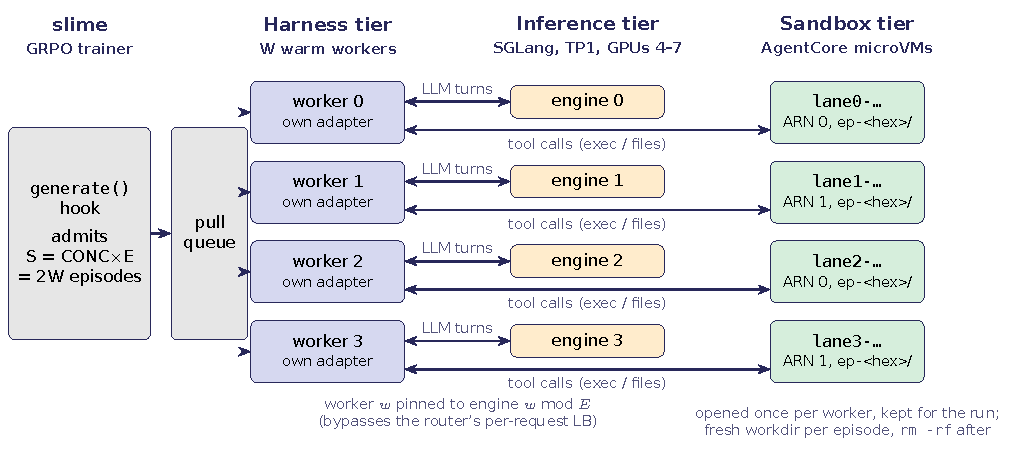
\includegraphics[width=0.92\textwidth,height=\textheight]{figures/lanes_fig01_lanes.pdf}}

\centerline{\emph{Figure 1: LANES = 4 → 4 workers : 4 engines : 4 persistent
microVMs.}}

\begin{itemize}
\tightlist
\item
  \texttt{LANES=N} sets all three tiers to N. \texttt{HARNESS\_WORKERS}
  alone moves only the harness tier.
\end{itemize}
\end{frame}

\begin{frame}[fragile]{Four mechanisms (\texttt{harness\_pool.py})}
\protect\hypertarget{four-mechanisms-harness_pool.py}{}
\begin{enumerate}
\tightlist
\item
  \textbf{Warm worker pool, pull-based.} W asyncio workers pull whole
  episodes from a shared queue (work-stealing): a worker stuck on a slow
  episode simply doesn't pull more.
\item
  \textbf{Engine pin.} At start-up each worker gets \textbf{its own
  \texttt{AnthropicAdapter}} pointed at engine \texttt{w\ mod\ E}
  (engines discovered from the router). All its turns hit one engine, so
  prefix-cache hits stay local. No slime patch.
\item
  \textbf{Persistent lane microVM.} Each worker opens \textbf{one}
  session
  (\texttt{lane\textless{}w\textgreater{}-\textless{}hex\textgreater{}},
  ARN \texttt{w\ mod\ K}) and keeps it for the run. Each episode gets a
  fresh \texttt{ep-\textless{}hex\textgreater{}} workdir, removed after.
  \texttt{LANE\_SANDBOX=0} restores a fresh session per episode.
\item
  \textbf{Admission sized to the lanes.} \texttt{CONC\ =\ ⌈2W\ /\ E⌉},
  so slime admits S = CONC × E = \textbf{2W} episodes: W being driven, W
  queued, so no worker idles between episodes.
\end{enumerate}
\end{frame}

\begin{frame}[fragile]{When a persistent VM is safe}
\protect\hypertarget{when-a-persistent-vm-is-safe}{}
\begin{longtable}[]{@{}
  >{\raggedright\arraybackslash}p{(\columnwidth - 4\tabcolsep) * \real{0.2292}}
  >{\raggedright\arraybackslash}p{(\columnwidth - 4\tabcolsep) * \real{0.3854}}
  >{\raggedright\arraybackslash}p{(\columnwidth - 4\tabcolsep) * \real{0.3854}}@{}}
\caption{Same AgentCore, opposite isolation choices}\tabularnewline
\toprule\noalign{}
\begin{minipage}[b]{\linewidth}\raggedright
\end{minipage} & \begin{minipage}[b]{\linewidth}\raggedright
scale\_lanes (this deck)
\end{minipage} & \begin{minipage}[b]{\linewidth}\raggedright
Terminal-Bench
\end{minipage} \\
\midrule\noalign{}
\endfirsthead
\toprule\noalign{}
\begin{minipage}[b]{\linewidth}\raggedright
\end{minipage} & \begin{minipage}[b]{\linewidth}\raggedright
scale\_lanes (this deck)
\end{minipage} & \begin{minipage}[b]{\linewidth}\raggedright
Terminal-Bench
\end{minipage} \\
\midrule\noalign{}
\endhead
What the agent changes & Files in its workdir & The whole OS: apt,
\texttt{/etc}, services \\
What the checker reads & Only the episode's workdir & System state \\
Reset & \texttt{rm\ -rf\ ep-\textless{}hex\textgreater{}/} (ms) & New
session = new microVM (boot) \\
Sessions per run & \textbf{W} (4) & \textbf{one per episode} (382) \\
Cold-start fix & Open once per lane & Look-ahead pre-open \\
\bottomrule\noalign{}
\end{longtable}

\textbf{The honest caveat:} the workers are asyncio tasks in one
process. They lift the \textbf{IO ceiling} (episodes are mostly waiting
on HTTP), not the \textbf{CPU ceiling}: the GIL still serialises
tokenisation and trajectory flattening. If profiling shows CPU-bound,
move to processes, not more coroutines.
\end{frame}

\hypertarget{results}{%
\section{5 · Results}\label{results}}

\begin{frame}[fragile]{Offline: the scaling law, measured
(\texttt{harness\_scaling\_demo.py})}
\protect\hypertarget{offline-the-scaling-law-measured-harness_scaling_demo.py}{}
\begin{longtable}[]{@{}
  >{\raggedright\arraybackslash}p{(\columnwidth - 12\tabcolsep) * \real{0.4783}}
  >{\raggedright\arraybackslash}p{(\columnwidth - 12\tabcolsep) * \real{0.0870}}
  >{\raggedright\arraybackslash}p{(\columnwidth - 12\tabcolsep) * \real{0.0870}}
  >{\raggedright\arraybackslash}p{(\columnwidth - 12\tabcolsep) * \real{0.0870}}
  >{\raggedright\arraybackslash}p{(\columnwidth - 12\tabcolsep) * \real{0.0870}}
  >{\raggedright\arraybackslash}p{(\columnwidth - 12\tabcolsep) * \real{0.0870}}
  >{\raggedright\arraybackslash}p{(\columnwidth - 12\tabcolsep) * \real{0.0870}}@{}}
\caption{Harness alone: plateau at the inference ceiling (40
ep/s)}\tabularnewline
\toprule\noalign{}
\begin{minipage}[b]{\linewidth}\raggedright
Harness-only sweep, W
\end{minipage} & \begin{minipage}[b]{\linewidth}\raggedright
1
\end{minipage} & \begin{minipage}[b]{\linewidth}\raggedright
2
\end{minipage} & \begin{minipage}[b]{\linewidth}\raggedright
4
\end{minipage} & \begin{minipage}[b]{\linewidth}\raggedright
6
\end{minipage} & \begin{minipage}[b]{\linewidth}\raggedright
\textbf{8}
\end{minipage} & \begin{minipage}[b]{\linewidth}\raggedright
12
\end{minipage} \\
\midrule\noalign{}
\endfirsthead
\toprule\noalign{}
\begin{minipage}[b]{\linewidth}\raggedright
Harness-only sweep, W
\end{minipage} & \begin{minipage}[b]{\linewidth}\raggedright
1
\end{minipage} & \begin{minipage}[b]{\linewidth}\raggedright
2
\end{minipage} & \begin{minipage}[b]{\linewidth}\raggedright
4
\end{minipage} & \begin{minipage}[b]{\linewidth}\raggedright
6
\end{minipage} & \begin{minipage}[b]{\linewidth}\raggedright
\textbf{8}
\end{minipage} & \begin{minipage}[b]{\linewidth}\raggedright
12
\end{minipage} \\
\midrule\noalign{}
\endhead
Throughput (ep/s) & 5.3 & 10.5 & 21.0 & 27.8 & \textbf{34.3} & 34.2 \\
Binding tier & harness & harness & harness & harness & \textbf{inf.} &
inf. \\
\bottomrule\noalign{}
\end{longtable}

\begin{longtable}[]{@{}lllll@{}}
\caption{All three tiers together: 8× tiers → 7.8×
throughput}\tabularnewline
\toprule\noalign{}
Balanced sweep, N + N + N & 1 & 2 & 4 & 8 \\
\midrule\noalign{}
\endfirsthead
\toprule\noalign{}
Balanced sweep, N + N + N & 1 & 2 & 4 & 8 \\
\midrule\noalign{}
\endhead
Throughput (ep/s) & 5.3 & 10.5 & 20.9 & \textbf{41.4} \\
\bottomrule\noalign{}
\end{longtable}

Real \texttt{run\_episode}, modelled tier ceilings, measured wall-clock.
Raising W alone stops paying once another tier binds; scaling
\textbf{jointly} stays near-linear.
\end{frame}

\begin{frame}[fragile]{AWS smoke run: lanes work (4 × 4 × 4,
2026-09-23)}
\protect\hypertarget{aws-smoke-run-lanes-work-4-4-4-2026-09-23}{}
\begin{longtable}[]{@{}
  >{\raggedright\arraybackslash}p{(\columnwidth - 2\tabcolsep) * \real{0.3711}}
  >{\raggedright\arraybackslash}p{(\columnwidth - 2\tabcolsep) * \real{0.6289}}@{}}
\caption{Smoke run (RB = 4, NS = 8, Qwen3-4B)}\tabularnewline
\toprule\noalign{}
\begin{minipage}[b]{\linewidth}\raggedright
Metric
\end{minipage} & \begin{minipage}[b]{\linewidth}\raggedright
Value
\end{minipage} \\
\midrule\noalign{}
\endfirsthead
\toprule\noalign{}
\begin{minipage}[b]{\linewidth}\raggedright
Metric
\end{minipage} & \begin{minipage}[b]{\linewidth}\raggedright
Value
\end{minipage} \\
\midrule\noalign{}
\endhead
Episodes / job & 400 over 10 steps + eval; job succeeded (≈ 24 min) \\
Lanes 1:1:1 (\texttt{check\_stickiness}) & ✓ every episode on its lane's
engine \textbf{and} lane's VM \\
Episodes per lane 0--3 & 103 / 101 / 99 / 97 (pull queue keeps them
balanced) \\
Session opens & \textbf{4} for the whole run (1.3--6.4 s each; 2 cold, 2
warm) \\
Warm sandbox ops (n = 2959) & p50 \textbf{80 ms}, p95 \textbf{120 ms}
(exec 98 · write 75 · read 73 ms p50) \\
Queue depth & p50 3, max 7 (≈ W queued, as admission intends) \\
Reward (train, per step) & 0.19 -- 0.50, mean 0.36 \\
Held-out \texttt{eval/deepscaler} & \textbf{0.358} at step 9 \\
\bottomrule\noalign{}
\end{longtable}
\end{frame}

\begin{frame}{Before / after: fresh session per episode vs lanes}
\protect\hypertarget{before-after-fresh-session-per-episode-vs-lanes}{}
\begin{longtable}[]{@{}
  >{\raggedright\arraybackslash}p{(\columnwidth - 4\tabcolsep) * \real{0.2889}}
  >{\raggedright\arraybackslash}p{(\columnwidth - 4\tabcolsep) * \real{0.3556}}
  >{\raggedright\arraybackslash}p{(\columnwidth - 4\tabcolsep) * \real{0.3556}}@{}}
\caption{Same task and harness; engine layout differs, so rollout time
is not a clean A/B}\tabularnewline
\toprule\noalign{}
\begin{minipage}[b]{\linewidth}\raggedright
\end{minipage} & \begin{minipage}[b]{\linewidth}\raggedright
Fresh session per episode (2026-09-18)
\end{minipage} & \begin{minipage}[b]{\linewidth}\raggedright
Lanes (2026-09-23)
\end{minipage} \\
\midrule\noalign{}
\endfirsthead
\toprule\noalign{}
\begin{minipage}[b]{\linewidth}\raggedright
\end{minipage} & \begin{minipage}[b]{\linewidth}\raggedright
Fresh session per episode (2026-09-18)
\end{minipage} & \begin{minipage}[b]{\linewidth}\raggedright
Lanes (2026-09-23)
\end{minipage} \\
\midrule\noalign{}
\endhead
Engines & 2 × TP2 & 4 × TP1 \\
Sandbox sessions opened & 400 (p50 0.41 s, Σ 177 s) & \textbf{4} (Σ 12
s) \\
Sandbox op p50 / \textbf{p95} & 90 / \textbf{431} ms & 80 / \textbf{120}
ms \\
Rollout time per step & 61 s & 64 s \\
Train reward / eval & 0.33 / 0.329 & 0.36 / 0.358 \\
\bottomrule\noalign{}
\end{longtable}

\begin{itemize}
\tightlist
\item
  The sandbox side improved as designed: \textbf{100× fewer opens, 3.6×
  lower p95}.
\item
  \textbf{Rollout time didn't move,} and that is the real finding (next
  slide).
\end{itemize}
\end{frame}

\begin{frame}{This workload is inference-bound}
\protect\hypertarget{this-workload-is-inference-bound}{}
\begin{itemize}
\tightlist
\item
  An episode takes ≈ \textbf{8 s} (64 s rollout ÷ 8 episodes per
  worker). The sandbox share is ≈ \textbf{0.65 s} (7.4 ops × 88 ms).
\item
  So \textbf{≈ 90 \% of an episode is SGLang generation}; the sandbox
  was never the bottleneck, and shaving it barely moves the step.
\item
  The 4 engines are also \textbf{under-used}: with 1 lane per engine,
  each engine serves \textasciitilde1 request at a time.
\end{itemize}

\textbf{Lesson:} a sandbox scaling demo needs a task where the
\textbf{sandbox does the work}. Math is the wrong task to show
AgentCore's elastic compute.
\end{frame}

\hypertarget{next-256-sandboxes-on-4-engines}{%
\section{6 · Next: 256 sandboxes on 4
engines}\label{next-256-sandboxes-on-4-engines}}

\begin{frame}[fragile]{Choosing a task the engines can keep up with}
\protect\hypertarget{choosing-a-task-the-engines-can-keep-up-with}{}
With N sandboxes in flight, each episode generating G tokens over T
seconds, the engines keep up only if

\textbf{N · G / T ≤ C} (C = aggregate decode rate of the 4 engines).

\begin{itemize}
\tightlist
\item
  Estimate C ≈ 10 k tok/s (Qwen3-4B, TP1 on L40S, batch
  \textasciitilde64 per engine; \textbf{to be measured}). With N = 256,
  G ≈ 1.5 k → \textbf{T ≥ 40 s}. Target 60--90 s of real sandbox CPU per
  episode for 2× headroom.
\item
  \textbf{Task: slow-verifier coding,} e.g.~performance optimisation.
  Short generations; each ``run tests'' is a heavy suite (property-based
  fuzzing, timed benchmark). Reward = tests passed + speed-up.
\item
  One knob, \texttt{EXEC\_BUDGET\_S}, sets the sandbox : inference
  ratio, so we can \textbf{move the bottleneck on purpose} and show the
  crossover.
\end{itemize}
\end{frame}

\begin{frame}[fragile]{Sizing the harness and slime}
\protect\hypertarget{sizing-the-harness-and-slime}{}
\begin{longtable}[]{@{}
  >{\raggedright\arraybackslash}p{(\columnwidth - 4\tabcolsep) * \real{0.1633}}
  >{\raggedright\arraybackslash}p{(\columnwidth - 4\tabcolsep) * \real{0.3265}}
  >{\raggedright\arraybackslash}p{(\columnwidth - 4\tabcolsep) * \real{0.5102}}@{}}
\caption{The 256-sandbox configuration}\tabularnewline
\toprule\noalign{}
\begin{minipage}[b]{\linewidth}\raggedright
Knob
\end{minipage} & \begin{minipage}[b]{\linewidth}\raggedright
Value
\end{minipage} & \begin{minipage}[b]{\linewidth}\raggedright
Why
\end{minipage} \\
\midrule\noalign{}
\endfirsthead
\toprule\noalign{}
\begin{minipage}[b]{\linewidth}\raggedright
Knob
\end{minipage} & \begin{minipage}[b]{\linewidth}\raggedright
Value
\end{minipage} & \begin{minipage}[b]{\linewidth}\raggedright
Why
\end{minipage} \\
\midrule\noalign{}
\endhead
Harness workers W & \textbf{256} (one per sandbox) & A worker drives one
episode at a time and mostly awaits exec: cheap \\
Layout & 4 lanes × 64 workers & Worker w → engine w mod 4 (prefix
cache); own persistent VM each \\
Adapters & \textbf{4} (one per engine) & Not 256 threads/servers;
workers share their engine's adapter \\
Harness CPU & ≈ 17 turns/s × 5--10 ms & ≤ 20 \% of a core: one process
is fine (profile to confirm) \\
\texttt{CONC} & ⌈2 · 256 / 4⌉ = 128 & slime admits 512: 256 driven + 256
queued \\
Batch & RB 64 × NS 8 = 512 / step & A queue refills stragglers at the
end of each step \\
Opens & 256 at ≤ 25/s ≥ 11 s, over K = 4--8 ARNs & New-session rate
quota {[}Q2{]}; 256 ≪ 5000 active \\
\bottomrule\noalign{}
\end{longtable}

\textbf{Proof:} sweep N = 32 / 64 / 128 / 256 at E = 4: throughput
should rise \textasciitilde linearly while SGLang running-requests and
per-call latency stay flat. Offline simulator first, then AWS.
\end{frame}

\begin{frame}{Takeaways}
\protect\hypertarget{takeaways}{}
\begin{itemize}
\tightlist
\item
  \textbf{AgentCore maps cleanly onto the sandbox tier:} Runtime =
  environment type, session = episode handle, microVM = isolation
  boundary.
\item
  \textbf{Isolation is a per-task choice:} persistent VM + fresh workdir
  for file-level tasks (this deck), fresh VM per episode for OS-level
  tasks (Terminal-Bench).
\item
  \textbf{Lanes work on AWS:} 1:1:1 verified, 4 opens instead of 400,
  sandbox p95 431 → 120 ms, reward and eval unaffected.
\item
  \textbf{Scale the bottleneck, not the tier you like:} math is
  inference-bound, so the next demo uses a sandbox-heavy task at 256 VMs
  to show where AgentCore's elastic CPU pays off.
\end{itemize}
\end{frame}

\begin{frame}[fragile]{References}
\protect\hypertarget{references}{}
\begin{longtable}[]{@{}
  >{\raggedright\arraybackslash}p{(\columnwidth - 4\tabcolsep) * \real{0.0545}}
  >{\raggedright\arraybackslash}p{(\columnwidth - 4\tabcolsep) * \real{0.5455}}
  >{\raggedright\arraybackslash}p{(\columnwidth - 4\tabcolsep) * \real{0.4000}}@{}}
\caption{References}\tabularnewline
\toprule\noalign{}
\begin{minipage}[b]{\linewidth}\raggedright
Ref
\end{minipage} & \begin{minipage}[b]{\linewidth}\raggedright
Source
\end{minipage} & \begin{minipage}[b]{\linewidth}\raggedright
Supports
\end{minipage} \\
\midrule\noalign{}
\endfirsthead
\toprule\noalign{}
\begin{minipage}[b]{\linewidth}\raggedright
Ref
\end{minipage} & \begin{minipage}[b]{\linewidth}\raggedright
Source
\end{minipage} & \begin{minipage}[b]{\linewidth}\raggedright
Supports
\end{minipage} \\
\midrule\noalign{}
\endhead
{[}Q1{]} & AgentCore quotas:
\url{https://docs.aws.amazon.com/bedrock-agentcore/latest/devguide/bedrock-agentcore-limits.html}
& Image ≤ 2 GB · 15-min idle timeout \\
{[}Q2{]} &
\texttt{aws\ service-quotas\ list-service-quotas\ -\/-service-code\ bedrock-agentcore}
(us-west-2, 2026-09-23) & Active sessions 5000 (L-3E5722B2) · new
sessions 25/s (L-8EE2AEA2) \\
{[}D3{]} &
\url{https://docs.aws.amazon.com/bedrock-agentcore/latest/devguide/runtime-how-it-works.html}
& Session = dedicated microVM; 15-min idle, 8 h max lifetime \\
Logs & \texttt{code/demos/\_smoke\_logs/lanes\_tb\_0923/scale\_lanes.*},
\texttt{\_smoke\_logs/demo\_cpu\_harness\_scale.*} & All measured
numbers in §5 \\
\bottomrule\noalign{}
\end{longtable}
\end{frame}

\end{document}
